\chapter{The PEMAN Structure}

The PEMAN structure is a hybrid photonic electronic structure which uses photonic operation for multiplication and electronic hardware for accumulation. It also has inbuilt non-linearity with the use of an ADC.

\section{Working Principle}

The PEMAN structure consists of three distinct sections: the analog photonics section, analog electronics section and digital electronic ssection. Each section applies one part of the ANN algorithm and is thus resuable inside a neural network. Each of the section is discussed in detail in the upcoming sections.

\subsection{Analog Photonics Section}

The analog photonics section is responsible for the multiplication of the input vector with the weight matrix. The multiplication of inputs and weights have been identified as the most computationally intensive part of the ANN algorithm and thus we can exploit photonics to the maximum extent by using it in this context.

In order to study how the multiplication works, a single MZI is first studied. Figure \ref{1x1mzi} shows the structure of an MZI.

\begin{figure}
	\centering
	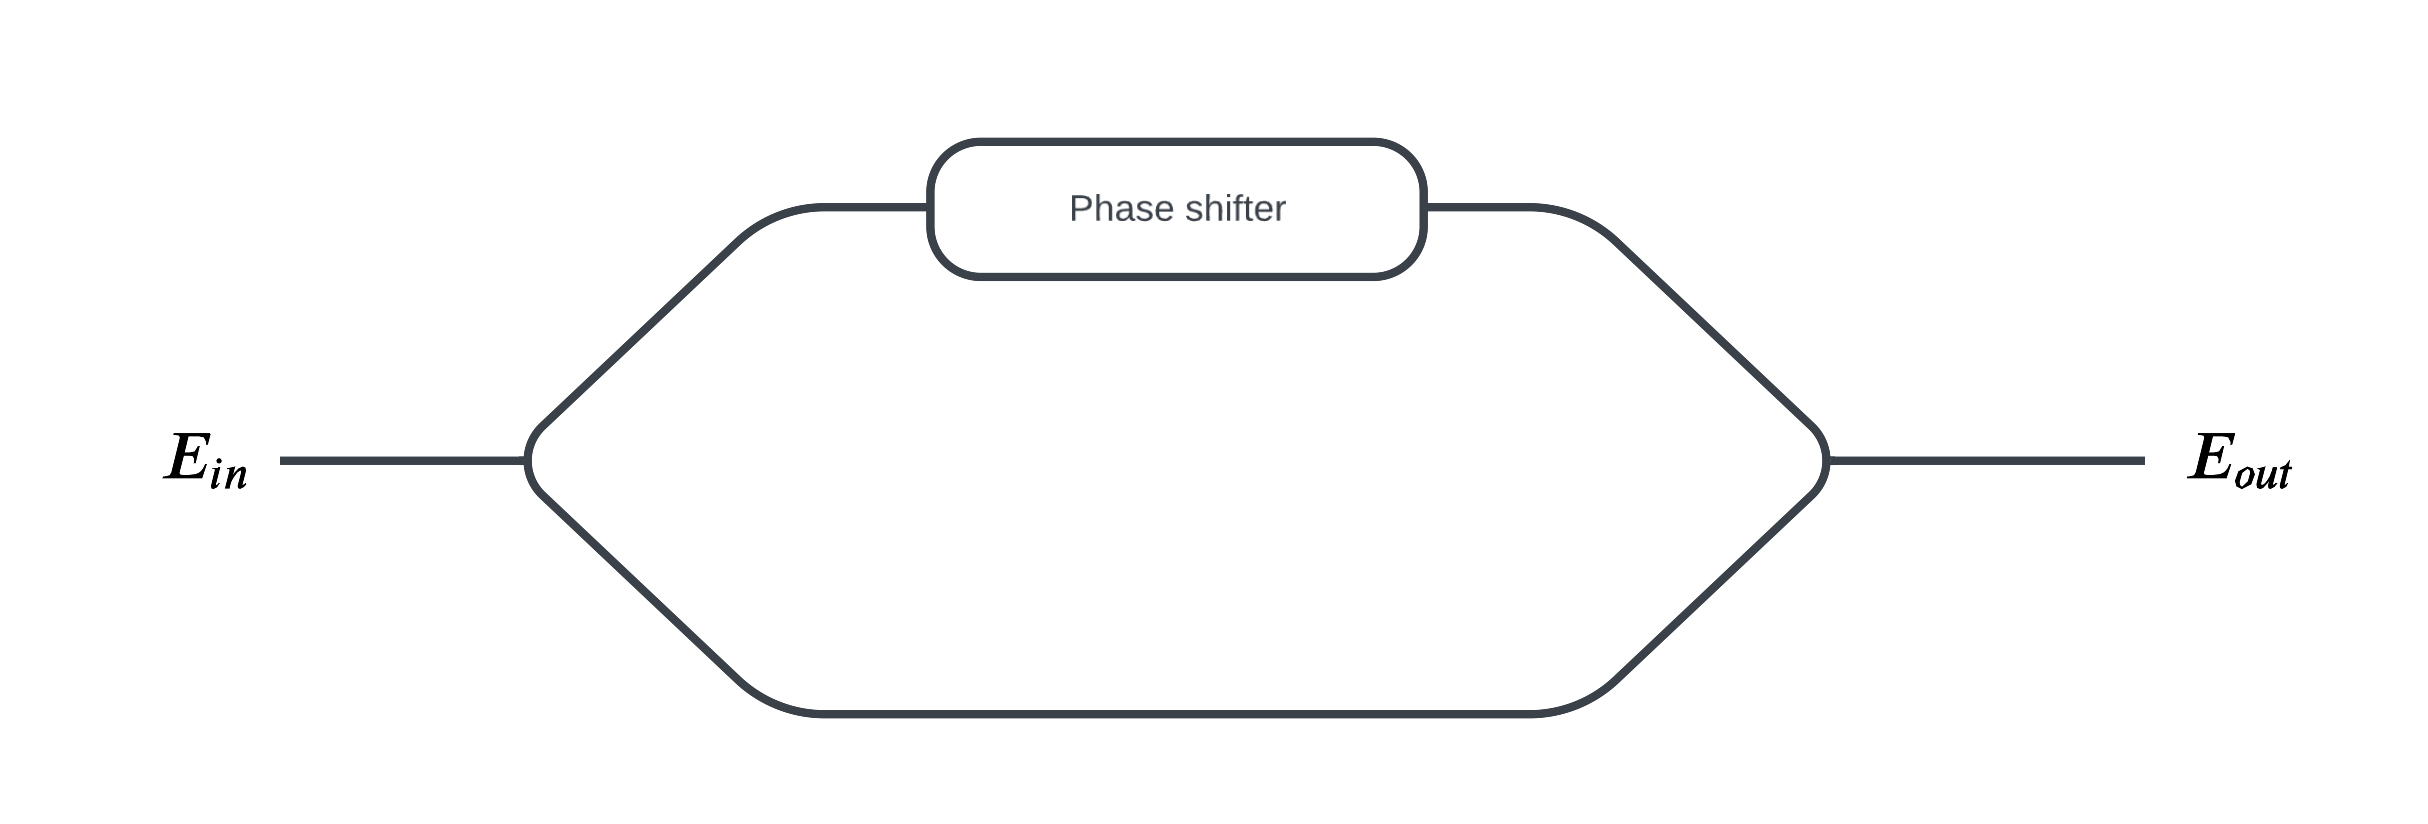
\includegraphics[width=\textwidth]{images/mzi.png}
	\caption{Schematic diagram of a 1x1 MZI}
	\label{1x1mzi}
\end{figure}

The structure is made up oftwo Y junctions on both sides with a phase shifter in-between. Lets say the input field is $E_{in}$, output field is $E_{out}$ and the phase shifter has a shift of is $\phi$. After applying the transfer matrices for each of the components, we get

\begin{equation}
	E_{out} = E_{in}\cos \phi
\end{equation}

This result can be interpreted as the multiplication of the input field with a value of $\cos \phi$. In PEMAN, the laser is generally given a constant current as it is reused for many operations. This means that the phase shifter needs to be changed dynamically to achieve multiplication.

In the actual PEMAN structure, two MZIs are used, one for input setting and one for weight setting, thereby giving the effect of multiplication of input and weight together.

Figure \ref{propPEMAN} depicts the structure that is used in this thesis as the PEMAN structure.

\begin{figure}
	\centering
	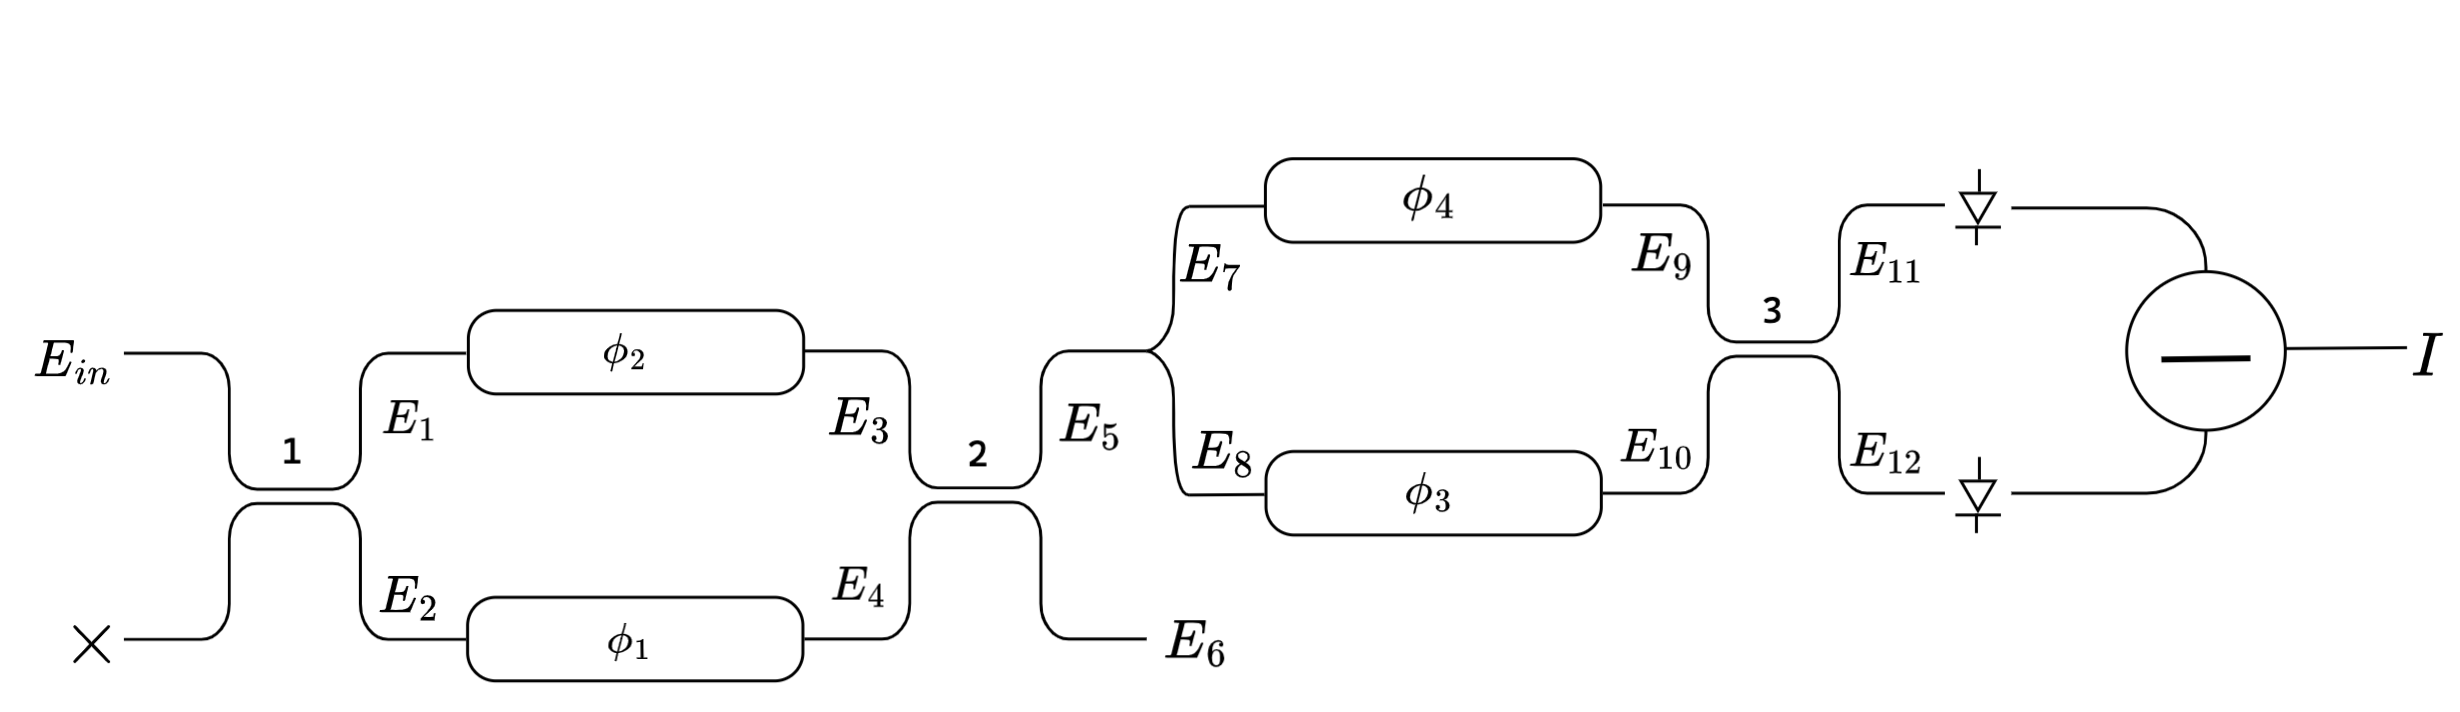
\includegraphics[width=\textwidth]{images/propPEMAN.png}
	\caption{Schematic diagram of the PEMAN structure}
	\label{propPEMAN}
\end{figure}

\subsection{Analog Electronics Section}

The analog electronics domain consists of a capacitor and a differential amplifier. These two components together is used as an accumulator to achieve the addition part in a neuron. Once the capacitor stores all the output produced by the photonics part, it is discharged into the next stage.

\subsection{Digital Electronics Section}

The digital electronics section consists of an ADC. This ADC is responsible to convert the analog current coming from the capacitor to digital domain. WHile converting, it is also implemented to apply a non- linear function to account for the activation function in a neuron. The ADC is also responsible for quantizing the output to a certain number of bits. Quantizing the values reduces the accuracy but boosts the overall speed.

\section{Timing Diagram}

Figure \ref{timing} shows the timing diagram of the PEMAN structure. The timing diagram shows the working of the PEMAN structure for a single neuron. It is necessary to study the time complexities and the under-workkings of the PEMAN structure in order to properly utilize its advantages.

\begin{figure}
	\centering
	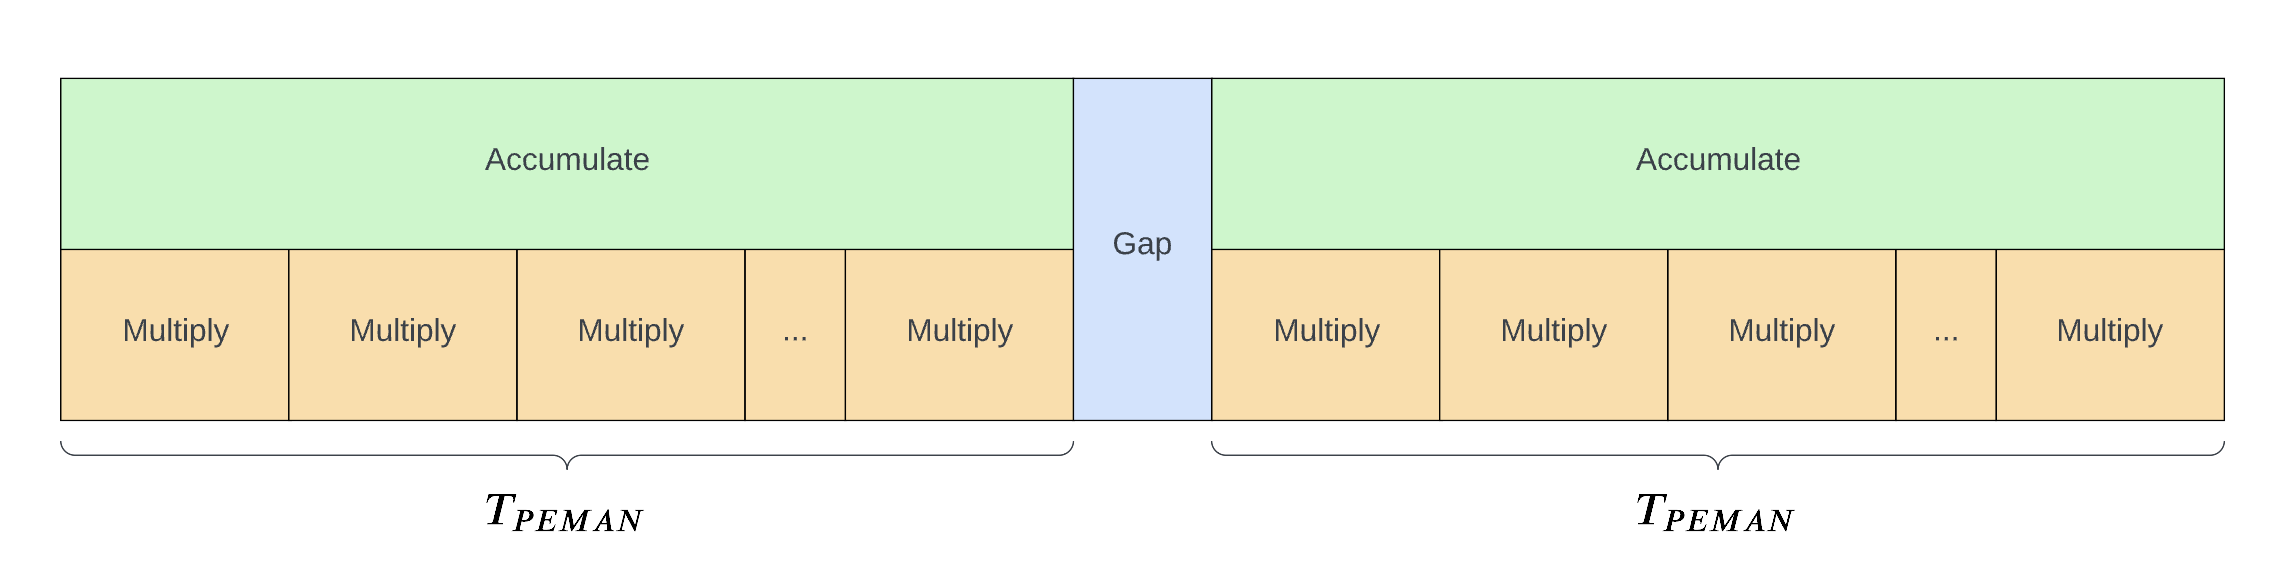
\includegraphics[width=\textwidth]{images/timing.png}
	\caption{Timing diagram of the PEMAN structure}
	\label{timing}
\end{figure}

From the figure, we can see that accumulation and the consecutive functions do not need to be as fast as multiplication. This is because multiplication is done a number of times before it has to be accumulated. This can also be leveraged by the fact that multiplication is done in the photonics domain and accumulation is done in the analog domain. This means that the multiplication can be done relatively fast while the accumulation can be done at a much slower speed.

\section{PEMAN Structure and Neural Networks}

The PEMAN structure is made to be reused such that an entire neural network can be implemented using the same structure. While it is implemented for the entire structure, we also need to consider training and inference.

\subsection{Conventional Method}

The conventional method to use a neural network built with the PEMAN structure involves using a GPU to train the model as normally done. Once the model has been trained to a satisfactory state, the weights are extracted. These weights are then matched with a premade lookup table to extract the necessary phase shifts for the weights. Now, when actual input is sent for inference, the inputs are converted to phases using the same lookup table, and set. The corresponding weight phases are set simultaneously. The output is then passed through the remainder of the structure and the final output is obtained.

This method is the traditional way to use PEMAN as we do not have to deal with reduced bit operation during training and can use effective quantization techniques to quantized the extract the weights without much drop in accuracy.

\subsection{Training on PEMAN}

Training on PEMAN is a relatively new concept. The idea is to train the model directly on the PEMAN structure. This means that the weights are not extracted from a GPU but are instead trained on the PEMAN structure itself. This is done by essentially using the same feedforward and backpropogation methods which are slightly modified to adapt to the new structure.

This approach can provide a significant speed boost to both training and inference as the weights do not need to be extracted and the entire model can be trained on the PEMAN structure itself. This also means that the model can be trained with reduced bit operation and thus can be trained faster. However, this approach is still in its infancy and needs to be studied in detail to understand its advantages and disadvantages.

One disadvantage might be that the reduced bit operation might degrade the accuracy more that necessary. But, upon testing for the handwritten digit recognition problem, it was found that the accuracy drop was not significant. This means that the reduced bit operation can be used to train the model faster without much drop in accuracy.

\section{Algorithm for training on PEMAN}

The process of training on PEMAN directly is fairly straightforward and bears a lot of resemblance to the original algorithm. The only real change is most of the operations now have an additional lookup step, which is necessary to convert the digital data to values of physical significance.

Figure \ref{trainOnPemanAlgo} shows the algorithm for training on PEMAN. The algorithm is divided into two parts: the feedforward part and the backpropogation part. The feedforward part is responsible for calculating the output of the network for a given input. The backpropogation part is responsible for calculating the gradients of the weights and biases and updating them.

\begin{figure}
	\centering
	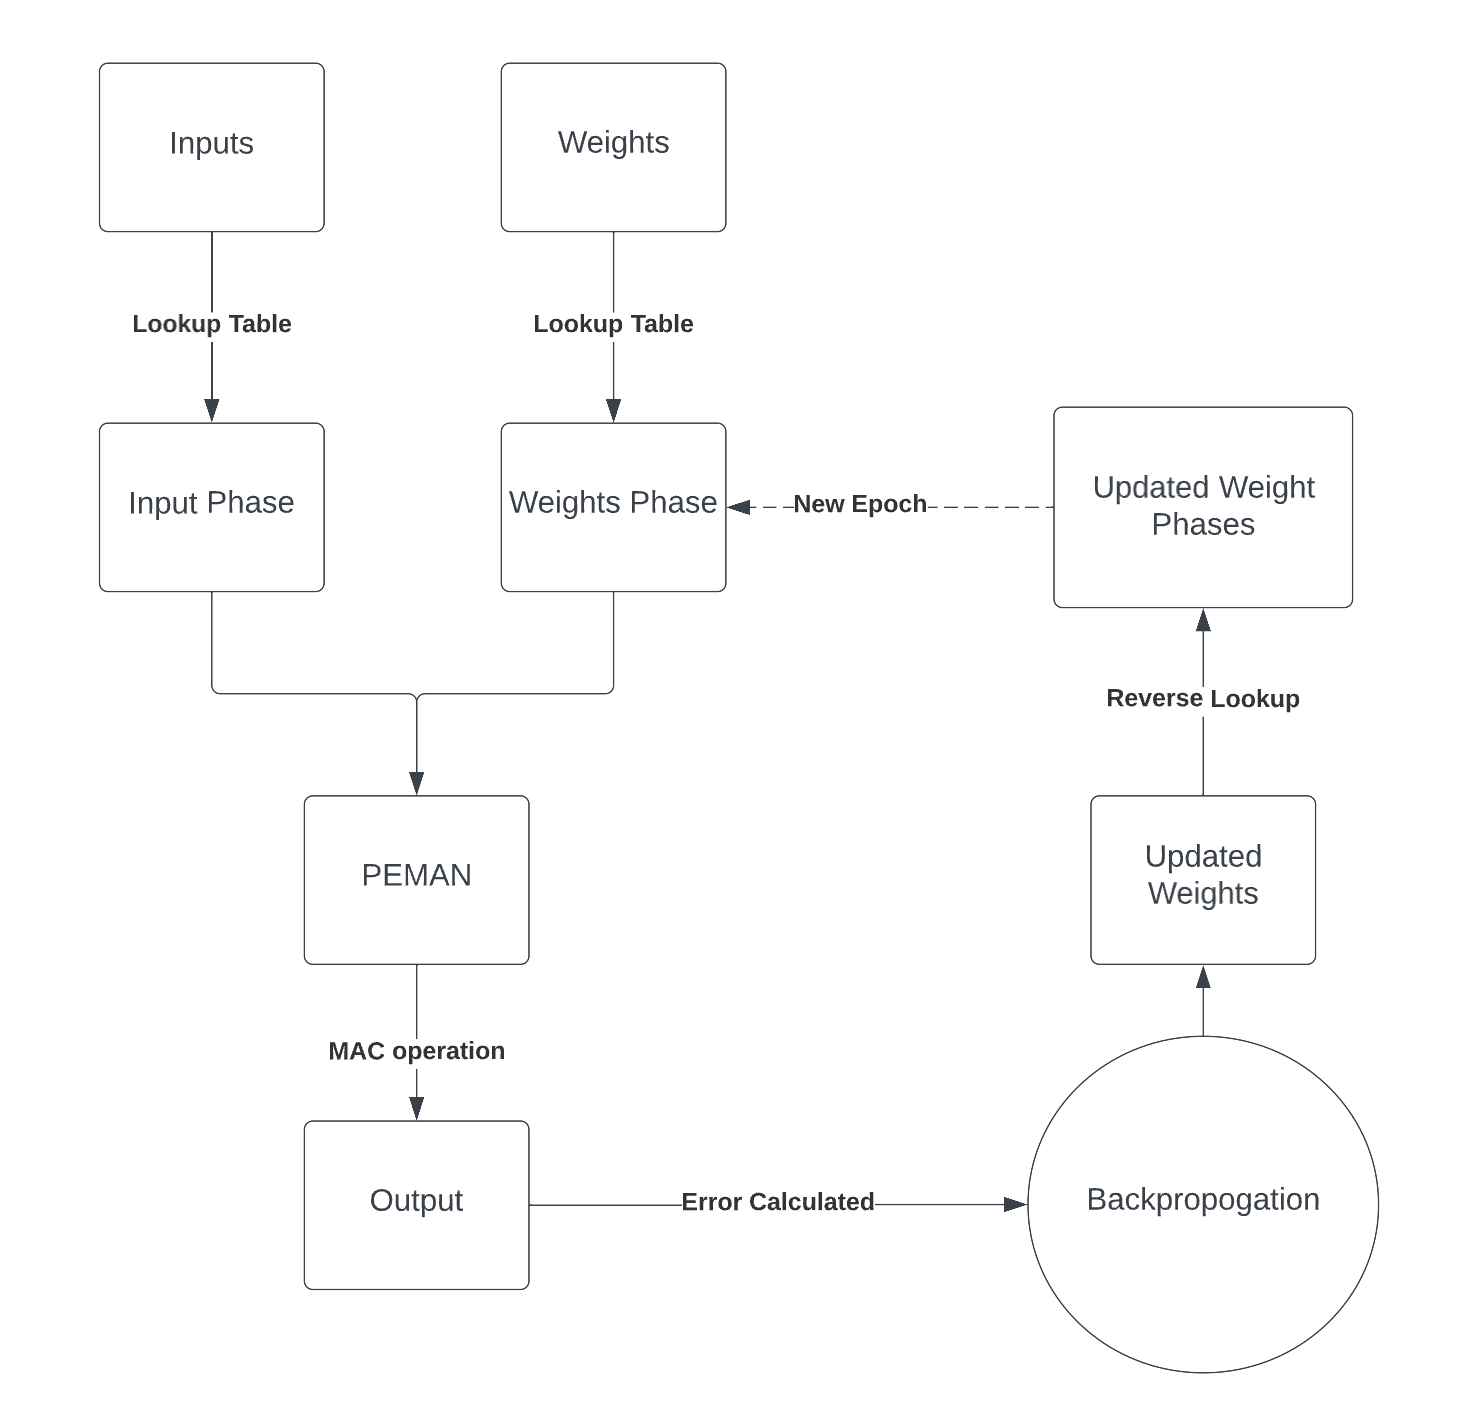
\includegraphics[width=\textwidth]{images/trainOnPemanAlgo.png}
	\caption{Algorithm for training on PEMAN}
	\label{trainOnPemanAlgo}
\end{figure}

Through using this technique, we employ the same backpropogation technique that has been proven to be successful while also modiying it so that we can train the phases of the PEMAN directly. This means that we can train the model directly on the PEMAN structure and thus can achieve a significant speed boost.

\section{PEMAN Structure and Handwritten Digit Recognition}

In order the study the practical implications of using such an approach, the handwritten digit recognition problem is used. The handwritten digit recognition problem is a classification problem where the goal is to classify a given handwritten digit into one of the 10 classes.

The complete flowchart as to how this entire training process takes place is illustrated in figure \ref{compFLowchart}.

\begin{figure}
	\centering
	\includegraphics[width=\textwidth]{images/compFLowchart.png}
	\caption{Complete flowchart of the training process using PEMAN}
	\label{compFLowchart}
\end{figure}

The dataset used for this problem is the MNIST dataset. The MNIST dataset consists of 60,000 training images and 10,000 testing images. The images are grayscale images of size 28x28. The dataset is split into training and testing sets with a ratio of 6:1.

The model used for this problem is a simple feedforward neural network with 1 hidden layer. The input layer has $28 \cdot 28 = 784$ parameters. The hidden layer has 100 parameters. The output layer has 10 parameters. The activation function used is the ReLU function. The loss function used is the cross entropy loss function. The optimizer used is the Adam optimizer. The model is trained for 10 epochs with a batch size of 64.

The model was trained in the same architecture but two different times. The first time, post training quantization technique was applied to quantize the wieghts to 8 bits and then the inference was run. In the second case, all the inputs and weights were quantized to various bit resolution while training itself. This helps us simulate the difference between training on PEMAN versus only inference through PEMAN.

The model when only done post-training quantization achieved an accuracy of 98.10\%. Figure \ref{trainingOnPeman} shows the accuracy values achieved by the same model when trained with pre-quantized parameters.

\begin{figure}
	\centering
	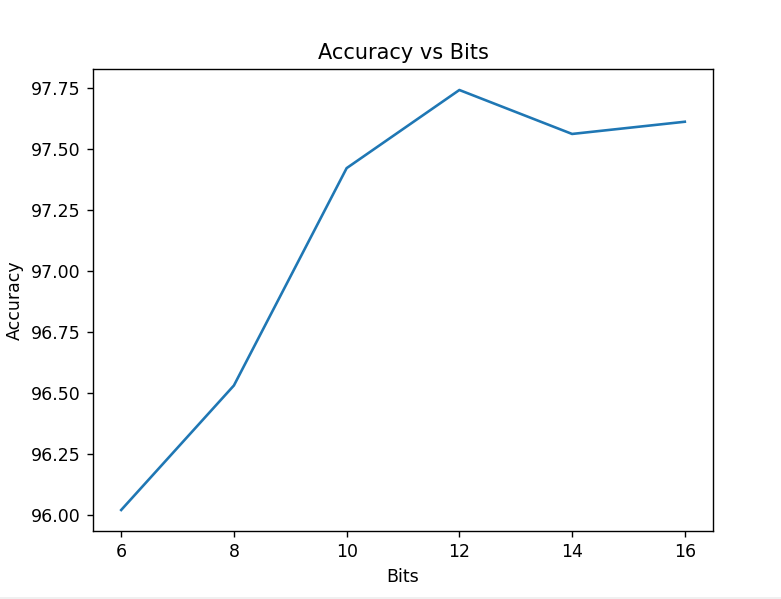
\includegraphics[width=\textwidth]{images/trainingOnPeman.png}
	\caption{Accuracy values achieved by the model when trained with pre-quantized parameters}
	\label{trainingOnPeman}
\end{figure}

From this plot, we can infer that at 8 bit resolution, we have an approximate accuracy of 96.50 \%, which is lower that 98.10\% achieved by the post-training quantization technique. However, we can also see that the accuracy is still quite high and the drop is not significant. This means that we can train the model with reduced bit operation and still achieve a high accuracy. This also means that we can train the model faster as the reduced bit operation is faster than the full bit operation.

